\documentclass[12 pt]{article}
\usepackage[top=1cm, left=1.5cm, right=1.5cm, bottom=1.5cm]{geometry}
\usepackage{graphicx, amsmath, tikz-cd, apacite, amssymb, tcolorbox, wrapfig}
\graphicspath{{./img/}}
\bibliographystyle{apacite}
\setlength{\parindent}{0pt}
\setlength{\parskip}{1em} 
 
\title{Introducción a las Transformaciones Lineales}
\author{Pablo Dario}
\date{03/01/2024}
 
\begin{document}
\maketitle

La diferencia entre una ecuación matricial $A\mathbf{x} = \mathbf{b}$ y la ecuación vectorial asociada ${x_1\mathbf{a_1} + \dots + x_n\mathbf{a_n}= \mathbf{b}}$ es tan solo cuestión de notación. Sin embargo, es posible encontrar una ecuación matricial $A\mathbf{x} = \mathbf{b}$ en álgebra lineal que no esté directamente relacionada con combinaciones lineales de vectores. Esto sucede cuando se piensa en la matriz A como un objeto que “actúa” sobre un vector $\mathbf{x}$ multiplicándolo para producir un nuevo vector $A\mathbf{x}$.
 
\begin{equation}
    \begin{aligned}
        & {\left[\begin{array}{rrrr}
        4 & -3 & 1 & 3 \\
        2 & 0 & 5 & 1
        \end{array}\right]\left[\begin{array}{l}
        1 \\ 1 \\ 1 \\ 1
        \end{array}\right]=\left[\begin{array}{l}
        5 \\ 8
        \end{array}\right] \text { y }\left[\begin{array}{rrrr}
        4 & -3 & 1 & 3 \\
        2 & 0 & 5 & 1
        \end{array}\right]\left[\begin{array}{r}
        1 \\ 4 \\ -1 \\ 3
        \end{array}\right]=\left[\begin{array}{l}
        0 \\ 0
        \end{array}\right]} \\
    \end{aligned}
\end{equation}

Así podemos observar que la multiplicación por la primera matriz transforma al primer vector en otro, y transforma al segundo vector en el vector cero.

\begin{figure}[ht]
  \centerline{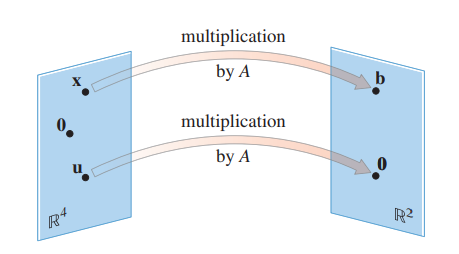
\includegraphics[width=0.4\textwidth]{image16.png}}
  \caption{Transformación de vectores por medio de multiplicación matricial}
\end{figure}

Así bien, desde este punto de vista resolver la ecuación $A\mathbf{x} = \mathbf{b}$ equivale a encontrar todos los vectores \textbf{x} en $\mathbb{R}^4$ que se transforman en el vector \textbf{b} en $\mathbb{R}^2$ como resultado de la acción de la multiplicación por $A$.

La correspondencia de \textbf{x} a $A$\textbf{x} es una \textbf{función} de un conjunto de vectores a otro. Este concepto generaliza la noción común de una función como una regla que transforma un número real en otro. Así bien una \textbf{transformación} puede verse como una \textbf{función o mapeo}.

Una \textbf{transformación} $T$ de $\mathbb{R}^n$ a $\mathbb{R}^m$ es una regla que asigna a cada vector \textbf{x} en $\mathbb{R}^n$ un vector $T$(\textbf{x}) en $\mathbb{R}^m$. El conjunto de $\mathbb{R}^n$ se llama \textbf{dominio} de $T$, y $\mathbb{R}^m$ se llama el \textbf{codominio} de $T$.\\ La notación $T$ : $\mathbb{R}^n \rightarrow \mathbb{R}^m$ indica que el dominio $T$ es $\mathbb{R}^n$ y que el codominio es $\mathbb{R}^m$. Para \textbf{x} en $\mathbb{R}^n$, el vector $T$(\textbf{x}) en $\mathbb{R}^m$ es la \textbf{imagen} de \textbf{x} (bajo la acción o transformación de $T$). El \textbf{conjunto de todas las imágenes} $T$(\textbf{x}) es el \textbf{rango} de $T$.

\begin{figure}[ht]
  \centerline{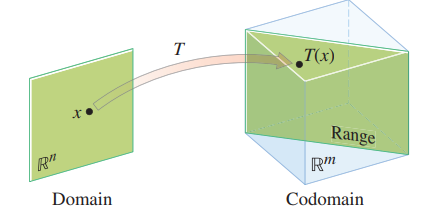
\includegraphics[width=0.4\textwidth]{image17.png}}
  \caption{Dominio, codominio y rango de $T$: $\mathbb{R}^n \rightarrow \mathbb{R}^m$}
  \label{}
\end{figure}

\begin{large}
    \textbf{Transformaciones Matriciales}
\end{large}

Para cada \textbf{x} en $\mathbb{R}^n$, $T$(\textbf{x}) se calcula como $A$\textbf{x}, donde $A$ es una matriz de $m \times n$. Para simplificar, algunas veces esta transformación matricial se denota como \textbf{x} $\longmapsto A$\textbf{x}. El dominio de $T$ es $\mathbb{R}^n$ cuando $A$ tiene $n$ columnas y el codominio de $T$ es $\mathbb{R}^m$ cuando las columnas de A tienen $m$ entradas. El rango de $T$ es el conjunto de todas las combinaciones lineales de las columnas de $A$ porque cada imagen $T$(\textbf{x}) es de la forma $A$\textbf{x}.

\begin{large}
    \textbf{Ejemplo 1}
\end{large}

\begin{wrapfigure}{r}{0.2\textwidth} 
    \centering
    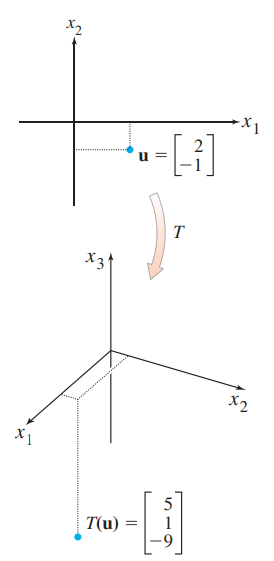
\includegraphics[width=0.2\textwidth]{image18.png}
    \caption{Imagen de \textbf{u}}
\end{wrapfigure}

Sean $A = \left[\begin{array}{rr}
    1 & -3 \\ 3 & 5 \\ -1 & 7
\end{array}\right]$, \textbf{u} $= \left[\begin{array}{r} 2 \\-1 \end{array} \right]$, \textbf{b} $= \left[\begin{array}{r} 3 \\ 2 \\ -5 \end{array} \right]$, \textbf{c} $= \begin{bmatrix} 3 \\ 2 \\5 \end{bmatrix}$  

defina una transformación $T: \mathbb{R}^2 \rightarrow \mathbb{R}^3$ por $T$(\textbf{x}) $= A$\textbf{x}, así bien obtenemos $$T(\mathbf{x}) = A\mathbf{x} = \left[\begin{array}{rr}
    1 & -3 \\ 3 & 5 \\ -1 & 7
\end{array}\right] \begin{bmatrix} x_1 \\ x_2 \end{bmatrix} = \left[\begin{array}{rr}
    x_1 & -3x_2 \\ 3x_1 & +5x_2 \\ -x_1 & +7x_2
\end{array}\right]$$

1.- Encuentre $T$(\textbf{u}), la imagen de \textbf{u} bajo la transformación de $T$ $$T(\mathbf{u}) = A\mathbf{u} = \left[\begin{array}{rr}
    1 & -3 \\ 3 & 5 \\ -1 & 7
\end{array}\right] \begin{bmatrix}
2 \\ -1
\end{bmatrix} = \left[\begin{array}{r}
    5 \\ 1 \\ -9
\end{array}\right]$$

2.- Encuentre una \textbf{x} en $\mathbb{R}^2$ cuya imagen bajo $T$ sea \textbf{b}

Para ello, debemos resolver $T$(\textbf{x}) = \textbf{b}. Es decir $A$\textbf{x} = \textbf{b} $$\left[\begin{array}{rr}
        1 & -3 \\ 3 & 5 \\ -1 & 7
\end{array}\right] \begin{bmatrix}
    x_1 \\ x_2
\end{bmatrix} = \left[\begin{array}{r}
        3 \\ 2 \\ -5
\end{array}\right]$$

Reducimos por filas la matriz aumentada:

\begin{equation*}
    \left[\begin{array}{rr|r}
    1 & -3 & 3 \\
    3 & 5 & 2 \\
    -1 & 7 & -5
    \end{array}\right] \sim\left[\begin{array}{rr|r}
    1 & -3 & 3 \\
    0 & 14 & -7 \\
    0 & 4 & -2
    \end{array}\right] \sim\left[\begin{array}{rr|r}
    1 & -3 & 3 \\
    0 & 1 & -.5 \\
    0 & 0 & 0
    \end{array}\right] \sim\left[\begin{array}{rr|r}
    1 & 0 & 1.5 \\
    0 & 1 & -.5 \\
    0 & 0 & 0
    \end{array}\right]
\end{equation*}

Así que $x_1 = 1.5, x_2 = -0.5$ y \textbf{x} $= \left[\begin{array}{c} 1.5 \\ -0.5 \end{array}\right]$ La imagen de este vector \textbf{x} bajo $T$ es el vector \textbf{b} dado

Ahora nos preguntamos si hay más de una \textbf{x} cuya imagen bajo $T$ sea \textbf{b} o bien ¿Es \textbf{b} la imagen de una única \textbf{x} en $\mathbb{R}^n$?; si vemos el vector anterior \textbf{x} nos daremos cuenta que no hay variables libres y por lo tanto la solución es única, es decir hay exactamente una \textbf{x} cuya imagen es \textbf{b}.

Para determinar si \textbf{c} está en el rango de la transformación $T$, debemos verificar si \textbf{c} es la imagen vectorial de alguna \textbf{x} en $\mathbb{R}^2$ es decir si $T$(\textbf{x}) = \textbf{c} para alguna \textbf{x}. Esto es otra manera de preguntar si el sistema $A$\textbf{x} = \textbf{c} es consistente. Al reducir la matriz aumentada obtenemos:

\begin{equation*}
    \left[\begin{array}{rr|r}
    1 & -3 & 3 \\
    3 & 5 & 2 \\
    -1 & 7 & 5
    \end{array}\right] \sim\left[\begin{array}{rr|r}
    1 & -3 & 3 \\
    0 & 14 & -7 \\
    0 & 4 & 8
    \end{array}\right] \sim\left[\begin{array}{rr|r}
    1 & -3 & 3 \\
    0 & 1 & 2 \\
    0 & 14 & -7
    \end{array}\right] \sim\left[\begin{array}{rr|r}
    1 & -3 & -3 \\
    0 & 1 & 2 \\
    0 & 0 & -35
    \end{array}\right]
\end{equation*}

La tercera ecuación nos indica que el sistema es inconsistente, por lo tanto \textbf{c} no está en el rango de $T$.

\begin{large}
    \textbf{Ejemplo 2}
\end{large}

Si $A = \begin{bmatrix}
    1 & 0 & 0 \\
    0 & 1 & 0 \\
    0 & 0 & 0
\end{bmatrix}$, entonces la transformación \textbf{x} $\longmapsto A$\textbf{x} proyecta puntos de $\mathbb{R}^3$ sobre el plano $x_1x_2$ porque 

\begin{equation*}
    \begin{bmatrix}
        x_1 \\ x_2 \\ x_3
    \end{bmatrix}
    \longmapsto \begin{bmatrix}
        1 & 0 & 0 \\
        0 & 1 & 0 \\
        0 & 0 & 0
    \end{bmatrix}
    \begin{bmatrix}
        x_1 \\ x_2 \\ x_3
    \end{bmatrix}
    = \begin{bmatrix}
        x_1 \\ x_2 \\ 0
    \end{bmatrix}
\end{equation*}

\begin{figure}[ht]
  \centerline{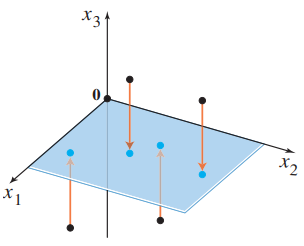
\includegraphics[width=0.3\textwidth]{image19.png}}
  \caption{Una transformación proyección}
\end{figure}

\begin{large}
    \textbf{Transformaciones Lineales}
\end{large}

Si $A$ es de $m \times n$ entonces la transformación \textbf{x} $\longmapsto A$\textbf{x} tiene las propiedades $$A(\mathbf{u} + \mathbf{v}) = A\mathbf{u} + A\mathbf{v} \quad \text{y} \quad A(c\mathbf{u}) = cA\mathbf{u}$$ para toda \textbf{u, v} en $\mathbb{R^n}$ y todos los escalares $c$

\begin{tcolorbox}[colback=red!10!white, colframe=red!70!black, title=Propiedades]
    Una transformación o (mapeo) $T$ es \textbf{lineal} si:
    \begin{itemize}
        \item[1.-] $T$(\textbf{u + v}) = $T$(\textbf{u}) + $T$(\textbf{v}) para todas las \textbf{u, v} en el dominio de $T$.
        \item[2.-]$T(c\mathbf{u}) = cT(\mathbf{u})$ para todos los escalares $c$ y para todas las \textbf{u} en el dominio de $T$. 
    \end{itemize}
\end{tcolorbox}

Cada transformación matricial es una transformación lineal; estas preservan las operaciones de suma vectorial y multiplicación escalar. Las propiedades anteriormente mencionadas conducen fácilmente a los siguientes útiles resultados

\begin{tcolorbox}[colback=blue!10!white,colframe=blue!60!black,title=Propiedades]
    Si $T$ es una transformación lineal, entonces $$T(0) = 0$$ y $$T(c \mathbf{u} + d \mathbf{v}) = cT(\mathbf{u}) + dT(\mathbf{v})$$
para todos los vectores \textbf{u, v} en el dominio de $T$ y para todos los escalares $c$, $d$.
\end{tcolorbox}

La segunda se puede generalizar, obteniendo $$T(c_1\mathbf{v_1} + \dotsb + c_p\mathbf{v_p}) = c_1T\mathbf{v_1} + \dotsb + c_pT\mathbf{v_p}$$ conocido también como principio de superposición.

\begin{large}
    \textbf{Ejemplo 3}
\end{large}

Dado un escalar $r$ defina $T: \mathbb{R}^2 \rightarrow \mathbb{R}^2$ por $T$(\textbf{x}) = $r$(\textbf{x}). $T$ se llama contracción cuando $0 \leq r \leq 1$ y una dilatación cuando $r > 1$. Sea $r = 3$ y demuetsre que $T$ es una Transformación lineal.

Sea \textbf{u} y \textbf{v} en $\mathbb{R}^2$ y sean $c, d$ escalares, obtenemos: $$ \begin{aligned}
    T(c\mathbf{u} + d\mathbf{v}) &= 3(c\mathbf{u} + d\mathbf{v})\\
    &= c(3\mathbf{u}) + d(3\mathbf{v})\\
    &= cT(\mathbf{u}) + cT(\mathbf{v})    
\end{aligned} $$

Así $T$ es una transformación lineal porque satisface $$T(c \mathbf{u} + d \mathbf{v}) = cT(\mathbf{u}) + dT(\mathbf{v})$$

\begin{figure}[ht]
  \centerline{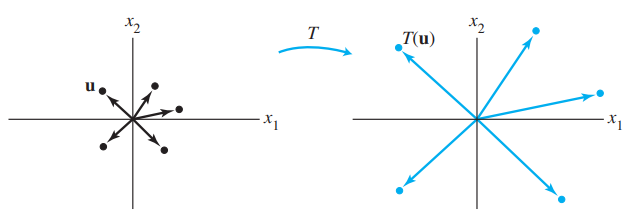
\includegraphics[width=0.45\textwidth]{image20.png}}
  \caption{Transformación de Dilatación}
\end{figure}

\pagebreak

\begin{large}
    \textbf{Ejemplo 4}
\end{large}

Defina una transformación $T: \mathbb{R}^2 \rightarrow \mathbb{R}^2$ mediante $$T(\mathbf{x}) = \left[\begin{array}{rr}
    0 & -1\\
    1 & 0
\end{array}\right] \begin{bmatrix}
    x_1 \\ x_2 
\end{bmatrix} = \left[\begin{array}{r}
    -x_2 \\ x_1
\end{array}\right] $$

Encuentre las imágenes bajo $T$ de \textbf{u} $= \begin{bmatrix}
    4 \\ 1
\end{bmatrix}, \mathbf{v} = \begin{bmatrix}
    2 \\ 3
\end{bmatrix}, \mathbf{u + v} = \begin{bmatrix}
    6 \\ 4
\end{bmatrix}$

Por lo tanto las Transformaciones quedarían de la siguiente manera: 
$$T(\mathbf{u}) = \left[\begin{array}{rr}
    0 & -1 \\
    1 & 0
\end{array}\right] \begin{bmatrix}
    4 \\ 1
\end{bmatrix} = \left[\begin{array}{r}
    -1 \\ 4
\end{array}\right]$$

$$T(\mathbf{v}) = \left[\begin{array}{rr}
    0 & -1 \\
    1 & 0
\end{array}\right] \begin{bmatrix}
    2 \\ 3
\end{bmatrix} = \left[\begin{array}{r}
    -3 \\ 2
\end{array}\right]$$

$$T(\mathbf{u + v}) = \left[\begin{array}{rr}
    0 & -1 \\
    1 & 0
\end{array}\right] \begin{bmatrix}
    6 \\ 4
\end{bmatrix} = \left[\begin{array}{r}
    -4 \\ 6
\end{array}\right]$$

Podemos observar que $T(\mathbf{u + v}) = T(\mathbf{u}) + T(\mathbf{v})$. Es claro que $T$ hace girar a \textbf{u, v} y \textbf{u + v} en el sentido antihorario en torno al origen en un ángulo de 90 grados. \cite{DavidC}

\begin{figure}[ht]
  \centerline{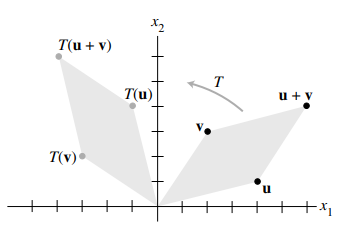
\includegraphics[width=0.3\textwidth]{image21.png}}
  \caption{Transformación de Rotación}
\end{figure}

\begin{tcolorbox}[colback=red!10!white, colframe=red!70!black, title=Resumen]
    \begin{itemize}
        \item[-] Una \textbf{transformación} $T$ de $\mathbb{R}^n$ a $\mathbb{R}^m$ es una regla que asigna a cada vector \textbf{x} en $\mathbb{R}^n$ un vector $T$(\textbf{x}) en $\mathbb{R}^m$.
        \item[-] El dominio de $T$ es $\mathbb{R}^n$ cuando $A$ tiene $n$ columnas y el codominio de $T$ es $\mathbb{R}^m$ cuando las columnas de A tienen $m$ entradas.
        \item[-] Los vectores que se van a transformar bajo $T$ de $\mathbb{R}^n$ a $\mathbb{R}^m$ tienen $n$ entradas y los vectores resultantes tienen $m$ entradas.
    \end{itemize}
\end{tcolorbox}

\bibliography{Referencias}

\end{document}